%匀速圆周运动的加速度(几何法)

\pentry{匀速圆周运动的速度(几何法)\upref{CMVG},加速度(矢量)\upref{VnA}}

在圆周运动中,位矢 $\vec r$ 是时间的函数.对时间求导后,我们得到速度矢量关于时间的函数.对速度也进行同样的操作,就不难得到圆周运动的加速度\upref{VnA}.
\begin{equation}
\vec a = \mathop {\lim }\limits_{\Delta t \to 0} \frac{\Delta \vec v}{\Delta t}
\end{equation}

现在我们用几何的方法来求该极限.根据矢量减法的定义% 未完成
,计算 $\Delta \vec v = {\vec v_2} - {\vec v_1}$ 要先把 ${\vec v_1}$ 和 ${\vec v_2}$ 的起点放在一起(例如都放在原点),再从 ${\vec v_1}$ 的终点指向 ${\vec v_2}$ 的终点得到 $\Delta \vec v$ (\autoref{CMAG_fig1}). 

\begin{figure}[ht]
\centering
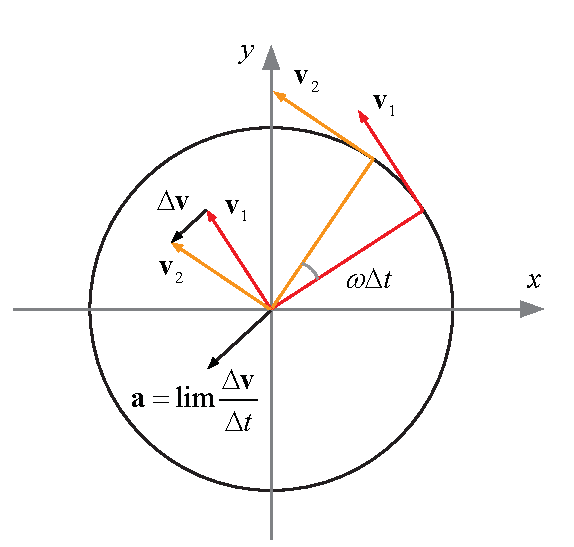
\includegraphics[width=7cm]{./figures/CMAG.pdf}
\caption{把速度矢量移到原点再相减}\label{CMAG_fig1}
\end{figure}

我们已知匀速圆周运动的速度大小为 $\abs{\vec v} = R\omega$, 根据“微小正弦极限\upref{LimArc}”中的结论,把 $\Delta\vec v$ 的长度用弧长近似,得
\begin{equation}
\abs{\Delta \vec v} = \abs{\vec v}\Delta \theta  = (R\omega)\omega \Delta t
\end{equation}
所以质点的加速度大小为
\begin{equation}
\abs{\vec a} = \lim_{\Delta t \to 0} \frac{(R\omega)\omega \Delta t}{\Delta t} = R{\omega ^2}\lim_{\Delta t \to 0} \frac{\Delta t}{\Delta t} = R{\omega ^2}
\end{equation}
由图可得加速度的方向是速度方向逆时针偏转 $\pi/{2}$. 又由于速度方向是位移方向逆时针偏转 $\pi/2$,所以\textbf{匀速圆周运动的加速度的方向与位矢的方向相反}.

结合模长和方向,令 $\vec r$ 为位矢,就得到加速度的矢量形式
\begin{equation}
\vec a =  - {\omega ^2}\vec r
\end{equation}


















